\chapter{Results and analysis}

\section{Classification improvements}

Results of classification accuracy of each classifier with each feature selection method on every possible subset of attributes was recorded during the experiments. The results are presented both in form of tables and plots. The tables showcases the best performance achieved by each feature selection method compared to full dataset. The plots illustrates accuracy of each feature selection method in respect to number of attributes.

Tables \ref{table:ANN}, \ref{table:NB} and \ref{table:SVM} show classification accuracy is improved or equal to the results of using a full set of features on all datasets tested. Only in naive Bayes \ref{table:NB} is there one dataset that performed better without feature selection.

% --- Tables ---
\begin{table}
  \begin{tabular}{|l|l|l|l|l|l|l|}
\toprule
{} & MIAS &   EN &  RHH & WBCD \\
\midrule
Chi2    & 0.58 & 0.59 & 0.64 & 0.71 \\
Entropy & 0.56 & 0.84 & 0.90 & 0.62 \\
SBS     & 0.54 & 0.55 & 0.59 & 0.74 \\
SFS     & 0.59 & 0.51 & 0.59 & 0.68 \\
Full    & 0.57 & 0.68 & 0.60 & 0.53 \\
Gain    & 0.04 & 0.24 & 0.51 & 0.41 \\
\bottomrule
\end{tabular}
 \\
  \caption{Classification accuracy achieved by ANN was improved on all datasets by the use of some feature selection method}
  \label{table:ANN}
  \vspace{1em}

  \begin{tabular}{|l|l|l|l|l|}
\toprule
{} &    MIAS &      EN &     RHH &    WBCD \\
\midrule
Chi2    & 0.70000 & 0.69262 & 0.90196 & 0.96524 \\
Entropy & 0.53333 & 0.83214 & 0.91373 & 0.95905 \\
SBS     & 0.63333 & 0.67286 & 0.91307 & 0.95143 \\
SFS     & 0.66667 & 0.67286 & 0.91895 & 0.96524 \\
Full    & 0.76667 & 0.68786 & 0.89608 & 0.93714 \\
\bottomrule
\end{tabular}
 \\
  \caption{All datasets except MIAS benefited from feature selection using CART Decision Tree classifier}
  \label{table:CART}
  \vspace{1em}

  \begin{tabular}{|l|l|l|l|l|}
\toprule
{} &    MIAS &      EN &     RHH &    WBCD \\
\midrule
Chi2    & 0.76667 & 0.74071 & 0.93693 & 0.95905 \\
Entropy & 0.76667 & 0.54810 & 0.91373 & 0.96524 \\
SBS     & 0.43333 & 0.70738 & 0.91307 & 0.97286 \\
SFS     & 0.43333 & 0.70738 & 0.91307 & 0.97286 \\
Full    & 0.76667 & 0.65976 & 0.93693 & 0.95905 \\
\bottomrule
\end{tabular}
 \\
  \caption{Naive Bayes sees improvement or equivalent accuracy by feature selection on every dataset}
  \label{table:NB}
  \vspace{1em}

  \begin{tabular}{|l|l|l|l|l|l|l|}
\toprule
{} &    MIAS &      EN &     RHH &    WBCD & Row differences & Dataset diff \\
\midrule
Chi2    & 0.56667 & 0.72690 & 0.89641 & 0.62810 &         0.01429 &     -0.07500 \\
Entropy & 0.33333 & 0.83214 & 0.91373 & 0.62810 &        -0.09649 &      0.00452 \\
SBS     & 0.53333 & 0.68333 & 0.88431 & 0.92952 &         0.22672 &     -0.00172 \\
SFS     & 0.53333 & 0.68333 & 0.88431 & 0.92952 &         0.22672 &      0.16500 \\
Full    & 0.56667 & 0.72690 & 0.89641 & 0.61381 &         0.00000 &          nan \\
\bottomrule
\end{tabular}
 \\
  \caption{Classification accuracy achieved by SVM was improved or equivalent on every dataset with use of feature selection}
  \label{table:SVM}
\end{table}
% ---/Tables ---

Each plot \ref{fig:plots_chi2}, \ref{fig:plots_entropy}, \ref{fig:plots_sbs} and \ref{fig:plots_sfs} represents one feature selection method. The subplots i.e. \ref{fig:RHH_chi2} visualises the classification accuracy on one dataset in respect to number of features.

The general characteristic of every plot is that the ANN performs the worst of all the classifiers. The ANN also provides the least consistent results with strong fluctuations in the results.

Chi2 in combination reveals a loss in accuracy with CART when using more than 23 attributes as seen in plot \ref{fig:WBCD_chi2}. It indicates a preference of more attributes on the RHH dataset in \ref{fig:RHH_chi2}.

Feature selection by Entropy shows clear performance on a subset compared to all features in \ref{fig:EN_entropy}. In plots \ref{fig:WBCD_entropy} and \ref{fig:RHH_entropy} the accuracy sees little to no improvement when increasing the number of attributes.

Using the wrapper method SBS both NB and ANN has an decrease in accuracy using all features in the EN dataset \ref{fig:EN_sbs}. However, both CART and SVM seems to prefer all features for an higher accuracy. In \ref{fig:WBCD_sbs} SVM has an strong decrease in performance using increasingly more features. CART and NB has a slight improvement using more features up to 27 where they starts to drop in there accuracy rate.  ANN has a very fluctuating scoring performance but has its highest accuracy using all features.  In the MIAS dataset using SBS shown in figure \ref{fig:MIAS_sbs} both SVM and NB prefers using all the features. ANN and CART has there highest performance using three features. In the plot \ref{fig:RHH_sbs} there seems to be an general trend that more features give an higher accuracy. CART drops slightly in accuracy at 9 or more features. NB drops in accuracy as well using the full dataset. ANN performs best using seven features.

The figure \ref{fig:plots_sfs} using SFS have a similar result to figure \ref{fig:plots_sbs} using SBS. The main differences are in \ref{fig:WBCD_sfs} where the best result for ANN is using only 24 features instead of the full dataset and in figure \ref{fig:RHH_sfs} where the best result for ANN have four features instead of seven.


% --- Plots ---
\begin{figure*}[htbp!]
  \centering
  \begin{subfigure}[b]{0.475\textwidth}
      \centering
      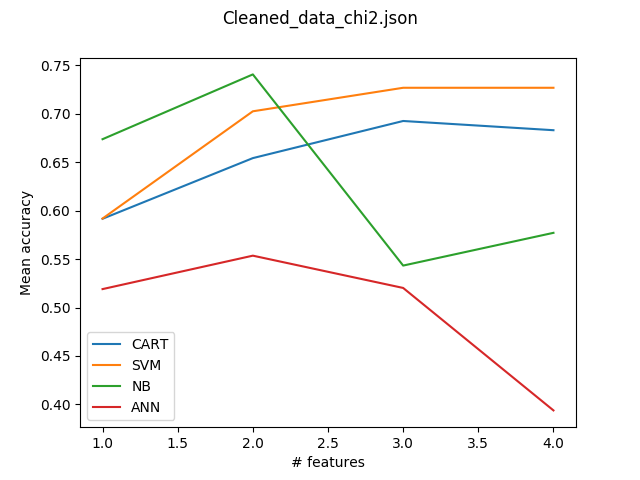
\includegraphics[width=\textwidth]{../plots_1d/Cleaned_data_chi2_combined.png}
      \caption[]%
      {{\small Dataset EN using Chi2}}
      \label{fig:EN_chi2}
  \end{subfigure}
  \hfill
  \begin{subfigure}[b]{0.475\textwidth}
      \centering
      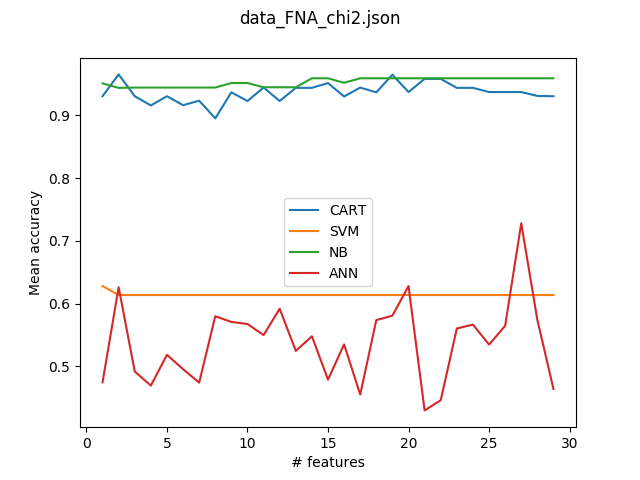
\includegraphics[width=\textwidth]{../plots_1d/data_FNA_chi2_combined.png}
      \caption[]%
      {{\small Dataset WBCD using Chi2}}
      \label{fig:WBCD_chi2}
  \end{subfigure}
  \vskip\baselineskip
  \begin{subfigure}[b]{0.475\textwidth}
      \centering
      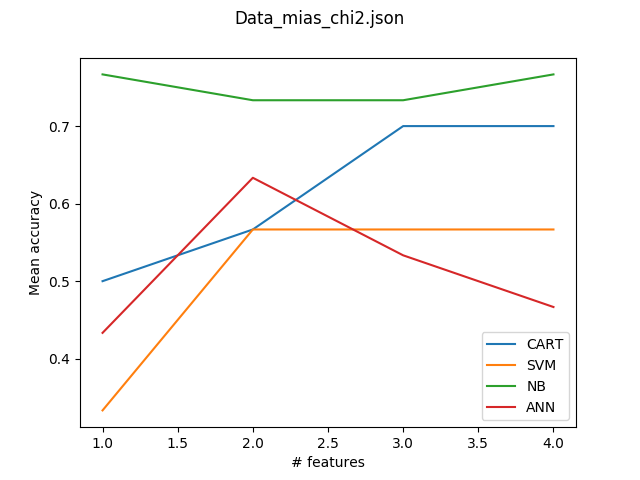
\includegraphics[width=\textwidth]{../plots_1d/Data_mias_chi2_combined.png}
      \caption[]%
      {{\small Dataset MIAS using Chi2}}
      \label{fig:MIAS_chi2}
  \end{subfigure}
  \quad
  \begin{subfigure}[b]{0.475\textwidth}
      \centering
      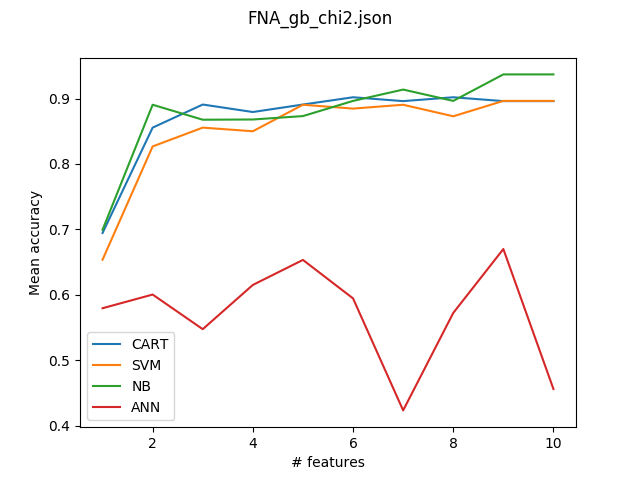
\includegraphics[width=\textwidth]{../plots_1d/FNA_gb_chi2_combined.png}
      \caption[]%
      {{\small Dataset RHH using Chi2}}
      \label{fig:RHH_chi2}
  \end{subfigure}

  \caption[ The average and standard deviation of critical parameters ]
  {Combined plots of all datasets comparing each classifier when using chi2 for feature selection.}
  \label{fig:plots_chi2}
\end{figure*}

\begin{figure*}[htbp!]
  \centering
  \begin{subfigure}[b]{0.475\textwidth}
      \centering
      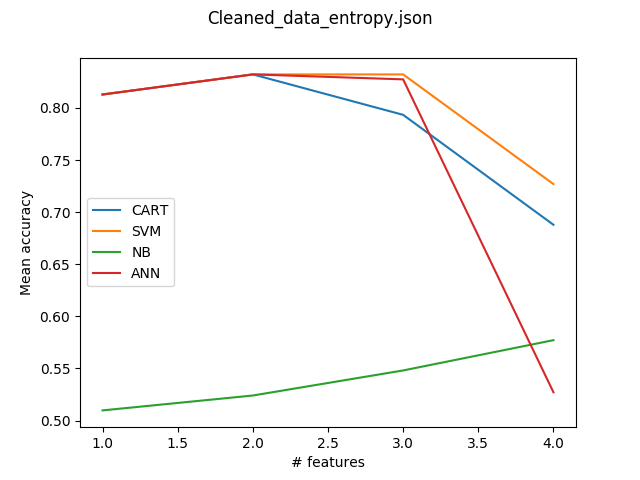
\includegraphics[width=\textwidth]{../plots_1d/Cleaned_data_entropy_combined.png}
      \caption[Network2]%
      {{\small Dataset EN using Entropy}}
      \label{fig:EN_entropy}
  \end{subfigure}
  \hfill
  \begin{subfigure}[b]{0.475\textwidth}
      \centering
      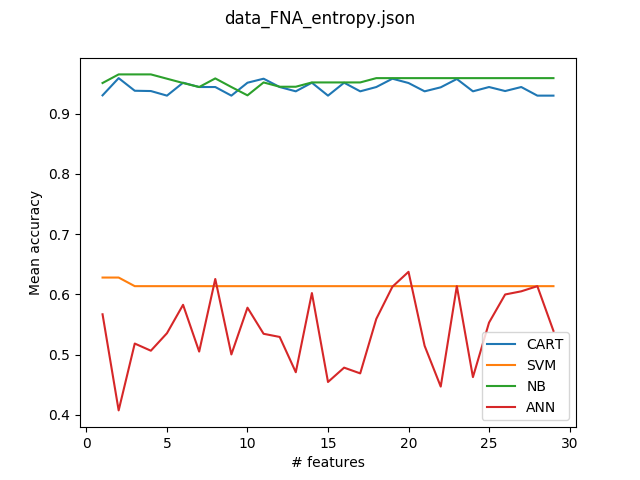
\includegraphics[width=\textwidth]{../plots_1d/data_FNA_entropy_combined.png}
      \caption[]%
      {{\small Dataset WBCD using Entropy}}
      \label{fig:WBCD_entropy}
  \end{subfigure}
  \vskip\baselineskip
  \begin{subfigure}[b]{0.475\textwidth}
      \centering
      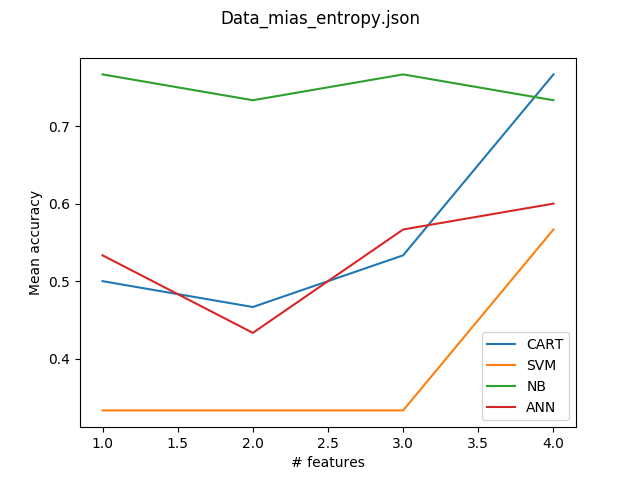
\includegraphics[width=\textwidth]{../plots_1d/Data_mias_entropy_combined.png}
      \caption[]%
      {{\small Dataset MIAS using Entropy}}
      \label{fig:MIAS_entropy}
  \end{subfigure}
  \quad
  \begin{subfigure}[b]{0.475\textwidth}
      \centering
      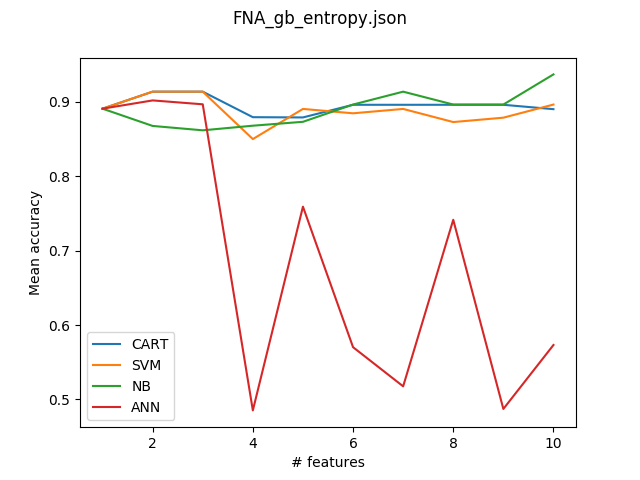
\includegraphics[width=\textwidth]{../plots_1d/FNA_gb_entropy_combined.png}
      \caption[]%
      {{\small Dataset RHH using Entropy}}
      \label{fig:RHH_entropy}
  \end{subfigure}
  \caption[]
  {{\small Combined plots of all datasets comparing each classifier when using Entropy for feature selection.}}
  \label{fig:plots_entropy}
\end{figure*}

\begin{figure*}[htbp!]
  \centering
  \begin{subfigure}[b]{0.475\textwidth}
      \centering
      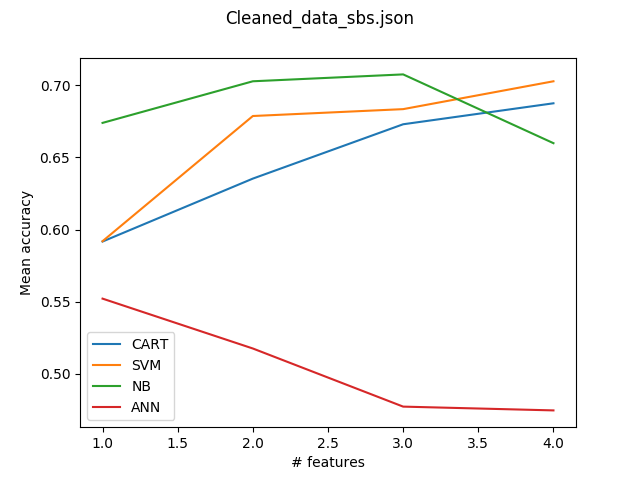
\includegraphics[width=\textwidth]{../plots_1d/Cleaned_data_sb_combined.png}
      \caption[]%
      {{\small Dataset EN using SBS}}
      \label{fig:EN_sbs}
  \end{subfigure}
  \hfill
  \begin{subfigure}[b]{0.475\textwidth}
      \centering
      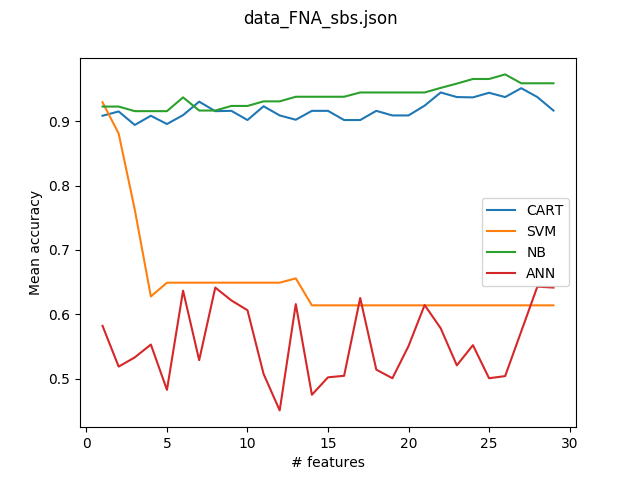
\includegraphics[width=\textwidth]{../plots_1d/data_FNA_sb_combined.png}
      \caption[]%
      {{\small Dataset WBCD using SBS}}
      \label{fig:WBCD_sbs}
  \end{subfigure}
  \vskip\baselineskip
  \begin{subfigure}[b]{0.475\textwidth}
      \centering
      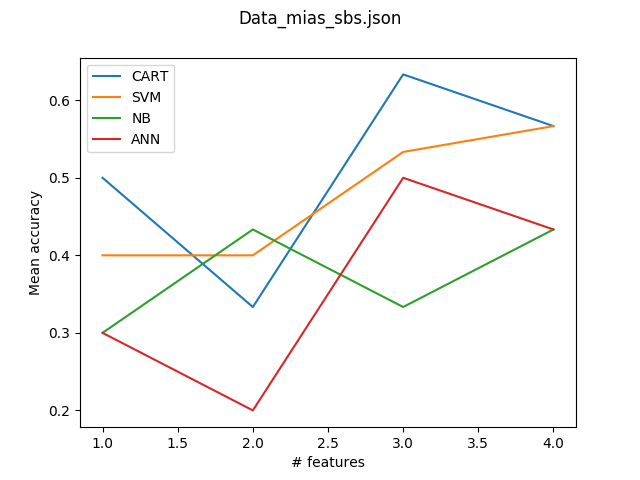
\includegraphics[width=\textwidth]{../plots_1d/Data_mias_sb_combined.png}
      \caption[]%
      {{\small Dataset MIAS using SBS}}
      \label{fig:MIAS_sbs}
  \end{subfigure}
  \quad
  \begin{subfigure}[b]{0.475\textwidth}
      \centering
      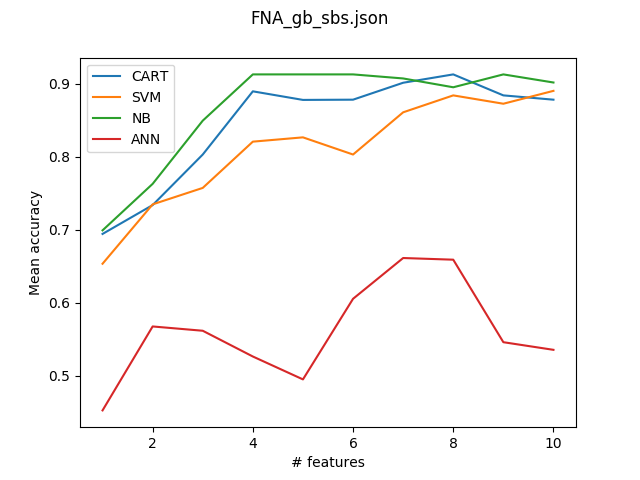
\includegraphics[width=\textwidth]{../plots_1d/FNA_gb_sb_combined.png}
      \caption[]%
      {{\small Dataset RHH using SBS}}
      \label{fig:RHH_sbs}
  \end{subfigure}
  \caption[]
  {{\small Combined plots of all datasets comparing each classifier when using SBS for feature selection.}}
  \label{fig:plots_sbs}
\end{figure*}

\begin{figure*}[htbp!]
  \centering
  \begin{subfigure}[b]{0.475\textwidth}
      \centering
      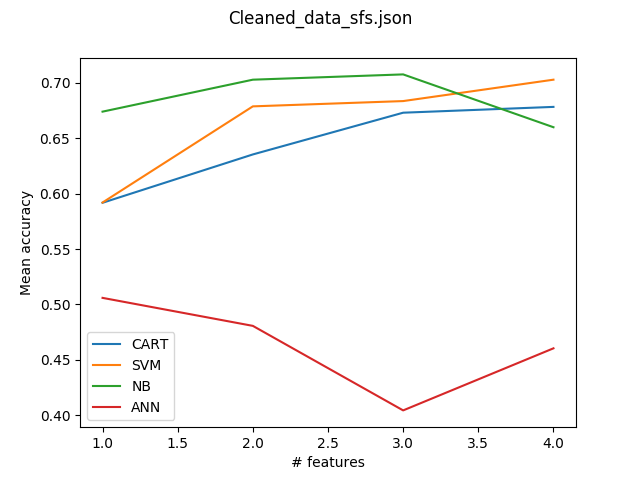
\includegraphics[width=\textwidth]{../plots_1d/Cleaned_data_sf_combined.png}
      \caption[]%
      {{\small Dataset EN using SFS}}
      \label{fig:EN_sfs}
  \end{subfigure}
  \hfill
  \begin{subfigure}[b]{0.475\textwidth}
      \centering
      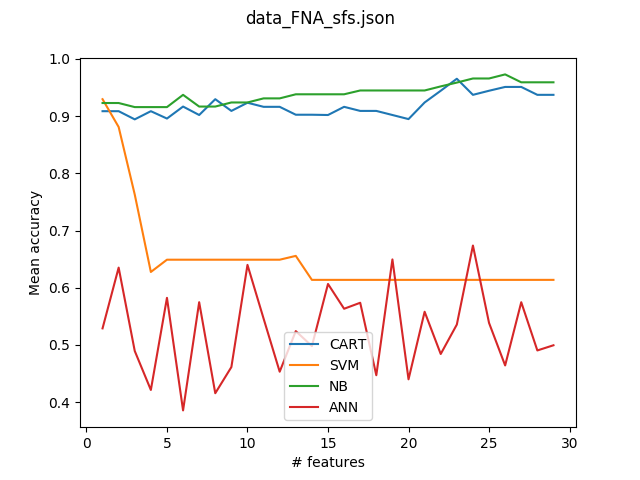
\includegraphics[width=\textwidth]{../plots_1d/data_FNA_sf_combined.png}
      \caption[]%
      {{\small Dataset WBCD using SFS}}
      \label{fig:WBCD_sfs}
  \end{subfigure}
  \vskip\baselineskip
  \begin{subfigure}[b]{0.475\textwidth}
      \centering
      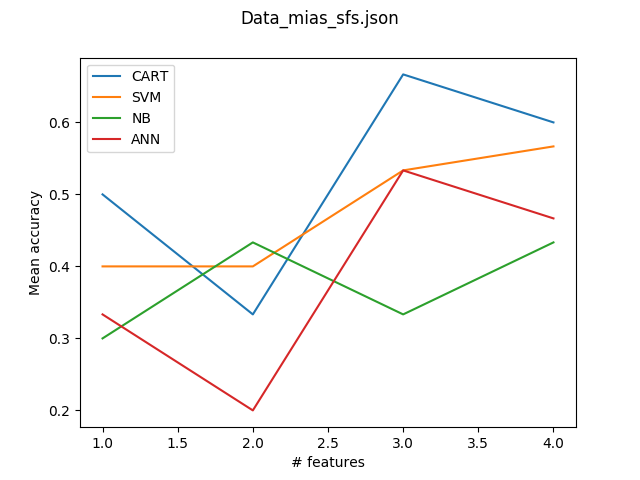
\includegraphics[width=\textwidth]{../plots_1d/Data_mias_sf_combined.png}
      \caption[]%
      {{\small Dataset MIAS using SFS}}
      \label{fig:MIAS_sfs}
  \end{subfigure}
  \quad
  \begin{subfigure}[b]{0.475\textwidth}
      \centering
      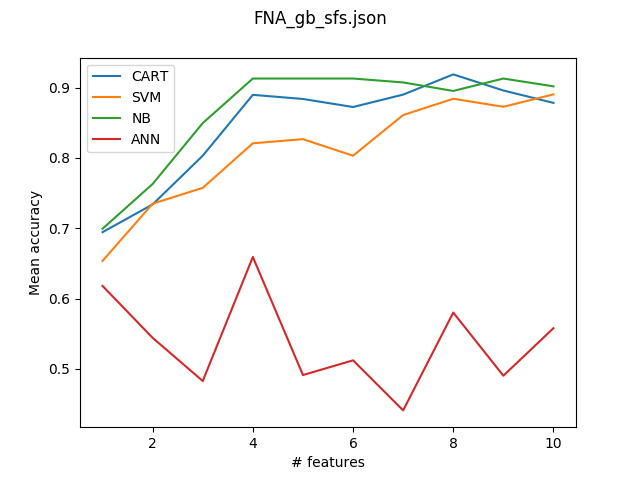
\includegraphics[width=\textwidth]{../plots_1d/FNA_gb_sf_combined.png}
      \caption[]%
      {{\small Dataset RHH using SFS}}
      \label{fig:RHH_sfs}
  \end{subfigure}
  \caption[]
  {{\small Combined plots of all datasets comparing each classifier when using SFS for feature selection.}}
  \label{fig:plots_sfs}
\end{figure*}
% ---/Plots ---

\section{Source of errors}
\label{sec:source_of_errors}

There are two main factor that may risk propagate error into the results, libraries and datasets.

The libraries provide all functionality of the classifiers and the filter selection methods, thus a major part of the implementation. A implementation built upon faulty methods can not provide any significant results. We use two libraries. The Scikit library \parencite{scikit-learn} is well renowned widely used in both industry and research thus inspire confidence in its robustness. The mlxtend library is used for SBS and SFS methods and is still a open source with less coverage than Scikit \parencite{mlextend}. Still it has a active community and many release versions indicating it's well managed.

The datasets...
